 \chapter{Proposta: PSkel-MPPA}
\label{cha:proposta}

Esta seção apresenta as ideias fundamentais que irão embasar a proposta e implementação
da adaptação do \fw \pskel para o processador \mppa.

\section{Visão Geral}

Como dito anteriormente, diversas dificuldades prejudicam o desenvolvimento de aplicações para
processadores \textit{manycore}, tais como o \mppa. Neste projeto, será dado um enfoque para
uma classe de aplicações paralelas que seguem o padrão \stencil. Nesse sentido, adaptar
o \fw PSkel para esse processador trará benefícios claros, simplificando o desenvolvimento
de aplicações \stencil para o \mppa. O \fw fornecerá uma transparência
no particionamento de tarefas e dados para esse ambiente, liberando o desenvolvedor
da utilização de meios de comunicação via \noc. Além disso, aplicações já desenvolvidas para o
\fw poderão ser executadas no \mppa sem a necessidade de nenhuma alteração em seus códigos originais.

% \todo[inline]{Destacar o que consiste a proposta: 1) que classes serão alteradas? 2) como será feita a comunicação dos dados? 3) será feito uso de técnicas para divisão dos tiles? quais? 4) será dado foco somente para desempenho? ou consumo de energia também? Os resultados obtidos serão comparados com quais outras arquiteturas?}

Na implementação da proposta será necessário modificar classes já existentes
no \fw para suportar as características do \mppa. Devido à subdivisão da matriz de entrada
e a comunicação serem diferentes para o \mppa em relação à um comunicação
\cpu-\gpu, classes responsáveis por essas
operações devem ser modificadas, como, por exemplo, a classe que determina a estrutura
\textit{Stencil}. Além disso, a comunicação entre os processos mestre e escravo
do \mppa será feita utilizando portais de comunicação.

Mais especificamente, uma nova função responsável por subdividir a matriz
de entrada em pequenas partes (\textit{tiles}), será criada.
Os \textit{tiles} serão construídos seguindo uma técnica de \textit{tiling}
trapezoidal~\cite{meng11}, sendo enviados para o processo trabalhador seguindo um modelo de
escalonamento de tarefas do tipo \textit{round-robin}.
Para efetuar o envio dos \textit{tiles} será criado um portal de comunicação relacionado com
cada \textit{tile} da matriz de entrada.

A técnica trapezoidal permite o mestre enviar \textit{tiles} aumentados, isto é,
\textit{tiles} com uma borda maior, determinada por uma \textit{ghost zone}.
% Desta forma, o processo trabalhador poderá realizar mais de uma iteração sobre
% cada \textit{tile}, diminuindo o número de sincronizações entre os processos.
A Figura~\ref{fig:tiling} ilustra essa técnica, onde a \textit{ghost zone}
agrupa as iterações em estágios. Cada estágio realiza
operações sobre \textit{tiles} sobrepostos, denominados trapezóides.
Por fim, os trapezóides irão produzir um dado sem sobreposição ao final da
computação de todas as iterações.
Com esta técnica, é possível realizar mais iterações sobre o mesmo
\textit{tile}, diminuindo o número de comunicações entre processos.

Devido ao \textit{tile} ser acrescido de uma parte da matriz atribuída à outro
\textit{tile}, computações redundantes serão realizadas. O tamanho do
\textit{tile} aumentado pode trazer perda em desempenho em troca de um menor
número de comunicações entre os processos, isto é, quanto maior o número de
computações redundantes, menor o número de comunicações. Desta forma, as \textit{ghost zones}
fornecem uma relação custo-benefício entre computações redundantes e a redução de
comunicações entre processos.

\begin{figure}[h]
	\centering
    \caption{Esquemático da técnica de \textit{tiling} trapezoidal.}
    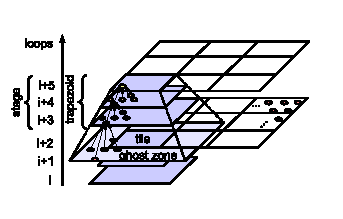
\includegraphics[width=0.6\textwidth]{figs/tiling.pdf}
    \caption*{Fonte: ~\cite{meng11}.}
    \label{fig:tiling}
\end{figure}

Os processos escravos deverão receber os
\textit{tiles} aumentados enviados pelo mestre, computar o \textit{kernel} da aplicação \stencil
sobre cada \textit{tile} e enviar o resultado ao mestre.
Além disso, será possível efetuar iterações sobre o mesmo \textit{tile},
buscando diminuir o número de comunicações. O \textit{kernel} da aplicação \stencil
será executado em paralelo em cada \textit{cluster} do \mppa, através do uso da \api OpenMP.

A implementação da proposta será focada em obter ganhos de desempenho e energia
em relação a outras arquiteturas, como, por exemplo, o processador
\textit{multicore} Intel Xeon. Desta forma, métodos escolhidos para efetuar a
comunicação e a subdivisão dos dados serão testados, buscando o melhor método
para cumprir o foco da proposta. 

\section{Trabalhos Relacionados}

A proposta deste trabalho está diretamente relacionada a diversos outros trabalhos de pesquisa.
A seguir, serão citados alguns trabalhos de pesquisa que fazem uso de esqueletos paralelos em
arquiteturas \textit{manycore}. Além disso, serão destacados alguns trabalhos de pesquisa sobre
o \mppa.

% \todo[inline]{Aqui, acho que poderia subdividir os trabalhos relacionados em subseções, de acordo com os assuntos que eles tratam.}

\subsection{Esqueletos paralelos e padrão \textit{stencil}}
\emph{Buono}~\etal~\cite{buono13} portaram um \fw baseado em esqueletos paralelos,
chamado de \emph{FastFlow}, para o processador \textit{manycore} \emph{TilePro64}.
Esse processador possui 64 núcleos de processamento idênticos, interconectados
por uma malha da \noc. O \fw \emph{FastFlow} provê padrões de \textit{design}
customizáveis, como, por exemplo, \textit{pipelines} e \textit{task farms},
que podem ser compostas para formar outros esqueletos, como \textit{map} e
\textit{reduce}.

De forma similar, \emph{Thorarensen}~\etal~\cite{thoraransen16} apresentaram um
novo \textit{back-end} do \fw \emph{SkePU} para o processador \textit{manycore}
de baixa potência \emph{Myriad2}. Esse processador possui uma arquitetura
heterogênea, tendo como alvo dispositivos com limites em questão de energia.
O \fw \emph{SkePU} provê uma interface de programação para esqueletos paralelos
como o \textit{map}, \textit{reduce}, e \textit{stencil}, com suporte para
diferentes \textit{back-ends}, incluindo processadores multicores e \gpus.

%------Trabalho relacionado sobre técnicas de tiling sobre o padrão estêncil.
%------Deixar para mencionar sobre trabalhos relacionados à isso.
\emph{Lutz}~\etal~\cite{lutz13} utilizaram técnicas de \textit{tiling} em
computações \textit{stencil} para lidar com a capacidade limitada de memória
de \gpus em ambientes multi-\gpu, utilizando as memórias das \gpus
coletivamente. De forma similar, \emph{Gysi}~\etal~\cite{gysi15} propuseram um \fw
para otimizações automáticas de \textit{tiling} em computações \textit{stencil}
situadas em um ambiente híbrido \cpu{}-\gpu.

%------------------------------------------

\subsection{Processadores \textit{manycore} de baixo consumo de energia}
Alguns trabalhos surgiram recentemente com intuito de avaliar o uso de
processadores \emph{manycore} em CAD, além de discutir os desafios do
desenvolvimento de aplicações para esses processadores.
Em~\cite{SCCEnergy:2012}, os autores compararam o desempenho e o consumo
energético de um processador \emph{manycore} experimental da Intel denominado
\emph{Single-Chip Cloud Computer} (SCC) com outros tipos de processadores e
GPUs. Para realizar essa análise, os autores utilizaram um conjunto de
aplicações paralelas implementadas em Charm++~\cite{Charm:2012}. Os resultados
obtidos com o Intel SCC mostraram que \emph{manycores} são uma alternativa
viável, apresentando bom desempenho e baixo consumo energético.
Em~\cite{MPPA-1:2013}, os autores avaliaram o desempenho do processador
\emph{manycore} MPPA-256 no contexto de aplicações de decodificação de vídeo. Os
resultados mostraram que o desempenho do MPPA-256 é comparável ao desempenho de
processadores Intel atuais em uma decodificação de vídeo no padrão H.264,
consumindo 6 vezes menos energia.

Trabalhos recentes revelaram o desempenho e consumo energético do processador
MPPA-256, comparando-o a outros processadores \textit{multicore} de propósito
geral e embarcados, no contexto de diferentes aplicações
científicas~\cite{Castro-SBAC-PAD:2014,Castro-IA3:2013,Castro-IA3-JPDC:2014}. Os
resultados mostraram que o processador \emph{manycore} MPPA-256 apresenta em
alguns casos desempenho superior a processadores \emph{multicore} Intel Xeon 2.4
GHz com 8 \emph{cores}, além de um consumo de energia de até 13 vezes menor em
relação ao mesmo processador. Um outro trabalho recentemente publicado realizou
uma análise comparativa de desempenho e consumo de energia entre processadores
\emph{multicore} Intel de alto desempenho e ARM~\cite{Castro-Padoin-IET:2015}.
Os resultados mostraram que, apesar da potência dos processadores ARM ser pelo
menos 10 vezes menor que a dos processadores Intel de alto desempenho, o consumo
de energia nem sempre será melhor, sendo dependente das características da carga
de trabalho a ser executada.

\emph{Morari}~\etal~\cite{Valero:2012} propuseram uma implementação otimizada do
\textit{radix sort} para o processador \textit{manycore} Tilera TILEPro64. Os
resultados mostraram que a solução para o TILEPro64 provê uma melhor eficiência
energética em relação à um processador \textit{multicore} de propósito geral, como
o Intel Xeon W5590, e em relação a uma \gpu NVIDIA Tesla C2070.

Mais especificamente, \emph{Francesquini}~\etal~\cite{Castro-IA3-JPDC:2014} analisaram
três diferentes classes de aplicações (CPU-\textit{bound}, \textit{memory-bound}
e híbrida) usando plataformas paralelas, como o \mppa, e um multiprocessador \numa de
192 núcleos e 24 nós. Mostrou-se que arquiteturas \textit{manycore} podem ser muito
competitivas, mesmo se a aplicação é, naturalmente, irregular. Os resultados mostraram
que o \mppa pode obter um desempenho maior (e um consumo de energia menor) que um
processador \textit{multicore} de propósito geral (Intel Xeon E5-4640) em um ambiente
com cargas de trabalho variadas e \cpu{}-\textit{bound}. Todavia, em um ambiente com cargas
de trabalho \textit{memory-bound}, o processador \numa obteve um melhor desempenho
em relação ao \mppa, apesar de apresentar também um maior consumo de energia.
Entre as plataformas avaliadas, o \mppa apresentou a melhor eficiência
energética, reduzindo a energia consumida em aplicações \cpu{}-\textit{bound},
híbridas e \textit{memory-bound} em 6.9x, 6.5x e 3.8x, respectivamente.

% Trabalhos recentes que propuseram APIs e ambientes de execução para
% \emph{manycores}. Em~\cite{TSHMEM:2013}, os autores propuseram uma adaptação
% Espaço de Endereçamento Global Particionado (\emph{Partitioned Global Address
%     Space} -- PGAS) para simplificar o desenvolvimento de aplicações paralelas
% para os processadores \emph{manycore} TILE-Gx e TILEPro. Mais precisamente, os
% autores utilizaram a biblioteca OpenSHMEM como base para a proposta,
% utilizando-a como uma camada de abstração para as bibliotecas fornecidas pelo
% fabricante dos processadores. Com isso, aplicações atualmente implementadas
% utilizando a API OpenSHMEM podem ser executadas nos processadores
% \emph{manycore} da linha TILE sem que haja a necessidade de modificações no
% código.
